% !TeX encoding = UTF-8
% !TeX program = xelatex
% !BIB program = bibtex
% !TeX spellcheck = en_US

\documentclass{cjc}

\usepackage{booktabs}
\usepackage{algorithm}
\usepackage{algorithmic}
\usepackage{siunitx}
\usepackage{listings}

\classsetup{
  % 配置里面不要出现空行
  title        = {浅谈区间操作及其数据结构},
  title*       = {Range Operations and their data structure},
  authors      = {
    author1 = {
      name         = {猫猫},
      name*        = {JIANG Wen-yuan},
      affiliations = {aff1},
      biography    = {男,同济大学本科在读。},
      % 英文作者介绍内容包括:出生年, 学位(或目前学历), 职称, 主要研究领域(与中文作者介绍中的研究方向一致).
      biography*   = {Undergraduate student at Tongji University.},
      email        = {1951510@tongji.edu.cn},
      %phone-number = {0},  % 第1作者手机号码(投稿时必须提供,以便紧急联系,发表时会删除)
    },
  },
  % 论文定稿后,作者署名、单位无特殊情况不能变更。若变更,须提交签章申请,
  % 国家名为中国可以不写,省会城市不写省的名称,其他国家必须写国家名。
  affiliations = {
    aff1 = {
      name  = {单位全名\ 部门(系)全名, 市(或直辖市) 国家名\ 邮政编码},
      name* = {Department of ****, University, City ZipCode, Country},
    },
  },
  abstract     = {
    中文摘要内容置于此处(英文摘要中要有这些内容),字体为小5号宋体。
    摘要贡献部分,要有数据支持,不要出现“...大大提高”、“...显著改善”等描述,
    正确的描述是“比…提高 X\%”、 “在…上改善 X\%”。
  },
  abstract*    = {Abstract (500英文单词,内容包含中文摘要的内容). },
  % 中文关键字与英文关键字对应且一致,应有5-7个关键词,不要用英文缩写
  keywords     = {关键词, 关键词, 关键词, 关键词},
  keywords*    = {key word, key word, key word, key word},
  %grants       = {
  %  本课题得到……基金中文完整名称(No.项目号)、
  %  ……基金中文完整名称(No.项目号)、
  %  ……基金中文完整名称(No.项目号)资助.
  %},
  % clc           = {TP393},
  doi           = {N/A},  % 投稿时不提供DOI号
  % received-date = {2019-08-10},  % 收稿日期
  % revised-date  = {2019-10-19},  % 最终修改稿收到日期,投稿时不填写此项
  % publish-date  = {2020-03-16},  % 出版日期
  % page          = 512,
}

\newcommand\dif{\mathop{}\!\mathrm{d}}

% hyperref 总是在导言区的最后加载
\usepackage{hyperref}

\lstset{basicstyle=\footnotesize\ttfamily,numberstyle=\tiny,numbers=none,frame=shadowbox}

\begin{document}

\maketitle

\section{引言}

\subsection{本文的目的}

在诸多软件工程的实践中,我们会经常遇到对一个线性数据结构的诸多连续区间进行操作的需求。“线性数据结构”和“连续区间操作”的概念可能略显抽象,下面的例子可以让你对这些概念有一个感性的认识。

例如,在一个列车购票系统中,列车可以依次停靠多个站台,且列车上的总座位数$S$是有限的。我们将站台编号为$1..n$,在从站台$k-1$到站台$k$的列车上的已占用座位数为$s[k]$。则乘客购票时,会提供其上车的站台$i$和下车的站台$j$,则该购票系统需要查询在$[i,j)$这个区间中,列车上已经占用的座位数量的最大值,即$\max_{k\in(i,j]}s[k]$。若该值恰好等于总座位数$S$,则系统不能接受该乘客的购票请求;反之,我们则接受该乘客的购票请求,并将$(i,j]$这个区间中的所有$s[k]$都加上$1$。

在上面的例子中,“线性数据结构”是指记录被编号的站台间列车上占用座位人数的$s[k]$,而“查询$\max_{k\in(i,j]}s[k]$”和“把$(i,j]$这个区间中的所有$s[k]$都加上$1$”就是对于一个连续区间的操作。实际的生产需要中,将时间或者某个方向的空间抽象为线性结构,并对线性结构上的区间进行一系列操作,是十分常见的(尤其在计算机图形学等领域)。因而,研究支持快速进行区间操作的数据结构显得十分具有价值。

然而,笔者在诸多关于数据结构的各层次教材中(从写给小朋友的算法书,到各类本科生的课程教材),关于这类数据结构介绍甚少,因而在本文中,笔者将一些支持区间操作的数据结构进行了不系统的整理,并对其应用场景和性能进行了分析,供同学们参考学习。

\subsection{区间信息}

在一个线性数据结构$s[k],(k\in [0,n))$中,我们称$[i,j],([i,j]\subseteq [0,n))$为一个区间。自变量为区间的一个函数$f_s(i,j)$为区间信息。例如:
\begin{equation*}
  f_s(i,j) = \sum_{i\leq x \leq j}^{}s[x]
\end{equation*}
\begin{equation*}
  f_s(i,j) = \max_{i\leq x \leq j}s[x]
\end{equation*}
\begin{equation*}
  f_s(i,j) = \frac{1}{i-j+1}\sum_{i\leq x \leq j}^{}s[x]
\end{equation*}
\begin{equation*}
  f_s(i,j) = \text{Xor} _{i\leq x \leq j}s[x]
\end{equation*}
均是区间信息。注意到计算区间信息时$s$中的数据没有发生变化,但是我们也将查询区间信息视为一种区间操作。

\subsection{区间操作}

除了计算一些区间信息外,对$s$中某段区间所存数据的批量修改是最常见的一种区间操作。本文中区间操作有如下的形式:
\begin{equation*}
  \text{Op} _s(i,j,F(x))
\end{equation*}
其中,$F(x)$是对区间每一个元素的操作。例如,将$[i,j]$区间中的每一个数都加上$a$、将$[i,j]$区间中的每一个数都进行平方、将$[i,j]$区间中的每一个数都设为$b$等,都是典型的区间操作。

\subsection{区间操作的性质}

常用的一些区间操作通常具有比较好的性质,可以用于简化问题的求解。其中,很多区间操作的性质可以和区间求和进行类比,我们记:
\begin{equation*}
  \text{sum\_range} _s(i,j) = \sum_{i\leq x \leq j}^{}s[x]
\end{equation*}
则不难证明,$\text{sum\_range} _s(i,j) = \text{sum\_range} _s(i,k) + \text{sum\_range} _s(k,j), k\in[i,j]$,即为区间的操作可以划分到子区间进行递归操作。求最大值、均值以及对区间进行加减乘除等赋值操作,均具有这样的性质。

另一种区间操作的性质被称为可重复贡献性质,这类性质是指对于区间信息的查询,有$x\, \text{opt}\, x = x$,即元素与自身做某个操作,仍然得到自身,例如$\max$和$\gcd$。而对于加和等操作,则没有这样的性质。

\subsection{一些约定}

本文为方便说明,仅考虑线性数据结构中的元素为正整数的情形。本文中的复杂度分析,均使用通常教材中的Big-O notation,即类似$O(n)$的表示方法。文中提供的代码片段的实现均使用C++或类似的伪代码写成,对于C++代码,遵循C++11标准。在复杂度的分析中,本着实用主义的理念,本文中将省略复杂度的证明。对于某些复杂度不十分显然的数据结构,本文采用事后测量的方式来验证理论所导出的复杂的的正确性,且主要考虑随机数据的情况。具体实现的程序见附录部分,且具体的测试数据见补充材料。

本文中有一些可能产生误解的名词,在这里约定其含义。

\paragraph{区间、区间信息和区间操作} 详见引言部分的说明。

\paragraph{在线算法和离线算法} 在计算机科学中,一个在线算法是指它可以以序列化的方式一个个的处理输入,也就是说在开始时并不需要已经知道所有的输入。相对的,对于一个离线算法,在开始时就需要知道问题的所有输入数据,而且在解决一个问题后就要立即输出结果。例如,选择排序在排序前就需要知道所有待排序元素,然而插入排序就不必。


\section{支持区间操作的数据结构}

下面我们将对一些常见的支持区间操作的数据结构进行分析。

\subsection{朴素的数组}

对于区间操作,一个最简单的想法就是按照其定义,对区间中的元素依次进行操作。例如,对于整数数组$s[n]$考虑以下几个操作:
\begin{enumerate}
  \item 求区间$[i,j]$的元素的和
  \item 求区间$[i,j]$的元素的最大值
  \item 将区间$[i,j]$中的每个元素都增加1
  \item 修改元素$s[i]$为$a$
\end{enumerate}
\subsubsection{实现方式}
利用数组存储这些元素,并用一个\lstinline{for}循环按照定义对每个元素进行计算即可,实现上十分简单且暴力。

\subsubsection{复杂度分析}
\paragraph{时间复杂度} 对于区间操作1、2、3,由于区间是随机给定的,故区间长度的期望正比于数组的大小,则每次操作的时间正比于区间长度,故对于每次操作,其复杂度为$O(n)$。而单点修改操作4,其复杂度仅为$O(1)$。
\paragraph{空间复杂度} 由于该数据结构没有引入额外的存储空间,因而其所占的内存为$O(n)$。
\subsubsection{适用范围与局限性}
由于没有引入任何优化,故该算法为在线算法,且支持几乎所有区间操作。
考虑m个请求,则处理所有这m个请求所需的时间复杂度为$O(mn)$,当$n$,$m$在同一个数量级时,其时间复杂度可视为$O(n^2)$,在数据量增大时,无疑是十分缓慢的。

\subsection{前缀数组}

如果我们只考虑对区间的查询操作,且查询操作具有类似加法一样可以差分的性质:
\begin{equation*}
  \text{sum\_range} _s(i,j) = \text{sum\_range} _s(k,j) - \text{sum\_range} _s(k,i)
\end{equation*}
\begin{equation*}
  k \leq i \leq j
\end{equation*}
我们则可以利用前缀数组进行高效的查询。公式里的求和与求差是抽象的,像求异或等操作,也具有类似的差分的性质。
\subsubsection{实现方式}
这里我们以查询区间$[i,j]$元素的和为例,另原数组为$s[n]$,引入前缀和数组$p[n]$,$p[n]$中元素$p[i]=s[0]+s[1]+s[2]+...+s[i]$。在实际实现中,使用$p[i]=p[i-1]+s[i]$,即可在一个\lstinline{for}循环中完成前缀数组的构建:
\begin{lstlisting}
p[0] = s[0];
for (int i = 1; i < n; i++)
{
    p[i] = p[i - 1] + s[i];
};
\end{lstlisting}
查询时,直接返回\lstinline{p[i]-p[j]+s[j]}即可。
\subsubsection{复杂度分析}
\paragraph{时间复杂度} 预处理时,构建前缀数组$p[n]$复杂度为$O(n)$。而区间查询操作,其复杂度仅为常数$O(1)$。如果对数据进行修改,则需重新建立前缀数组,复杂度为$O(n)$。
\paragraph{空间复杂度} 虽然该数据结构引入了额外的存储空间,但由于$p[n]$与$s[n]$大小同阶,故占用内存仍然为$O(n)$,只是常数略大。
\subsubsection{适用范围与局限性}
考虑m个请求,则处理所有这m个请求所需的时间复杂度为$O(m+n)$(包括预处理的时间),当$n$,$m$在同一个数量级时,其时间复杂度可视为$O(m)$,在数据量增大时,查询是十分快速的。

但该数据结构不支持对数据的高效修改,仅支持高效查询,属于离线的数据结构,且对于区间查询有差分性质的限制。

\subsection{ST表}
即使在不对区间进行修改的情况下,如果某种区间信息不具有差分的性质,也无法使用前缀数组进行高效的查询。ST表(Sparse Table,稀疏表)这类数据结构可以高效处理这类符合结合律且可重复贡献的区间信息查询问题。一种典型的这类问题被称为RMQ(Range Maximum/Minimum Query,区间最大/最小值查询)问题。
\subsubsection{实现方式}
以查询区间最大值为例,ST表使用一个二维数组$f(i,j)$存储区间区间$[i,i+2^j-1]$的最大值。

初始化时,首先有$f(i,0)=a_i$,其中$a_i$即是原数组中的$s[i]$。接下来利用动态规划的方式计算$f(i,j)$,由定义可知$f[i,j]=\max(f[i,j],f[i+2^{j-1},j])$。

查询时,对于每个询问的区间$[l,r]$,将其分为两个部分$[l,l+2^s-1]$与$[r-2^s+1,r]$,其中$s=\left \lfloor log_2 (r-l+1) \right \rfloor $通过查表可得$f[l,l+2^s-1]$与$f[r-2^s+1,r]$,则$max(f[l,l+2^s-1],f[r-2^s+1,r])$即为区间最大值。

\subsubsection{复杂度分析} 
\paragraph{时间复杂度} 对于预处理时$f[i,j]$的计算,计算的列数为$n$,而行数为$log_2\,n$,故其所耗时间为$O(n\, log \, n)$,而查询所用的时间为常数$O(1)$。
\paragraph{空间复杂度} 与$f[i,j]$所占空间一致,为$O(n\, log \, n)$。
\subsubsection{适用范围与局限性}

该数据结构不支持对数据的高效修改,仅支持高效查询(常数时间)。考虑m个请求,则处理所有这m个请求所需的时间复杂度为$O(m+n\, log \, n)$(包括预处理的时间),当$m$很大时,其时间复杂度可视为$O(m)$,应对大量查询是十分快速的。ST表属于离线的数据结构,且对于区间查询操作的信息需符合结合律且可重复贡献的性质。

\subsection{树状数组}
仍然考虑区间求和问题,为了克服前缀数组无法高效修改的局限性,我们引入了树状数组(Binary Index Tree, BIT),又称二进制下标树。
\subsubsection{实现方式}
朴素的数组的单点修改是$O(1)$,但是区间求和是$O(n)$。而前缀数组单点修改是$O(n)$,但是区间求和是$O(1)$。因此现在我们希望找到这样一种折中的方法:无论单点修改还是区间查询,它都能不那么慢地完成。

一个很自然的想法是,我们用一个数组$c$维护若干个小区间,单点修改时,只更新包含被修改元素的区间;在求区间和时,将$[0,i]$和$[0,j]$求出,用于前缀数组一样的方法计算$[i,j]$的和(差分即可)。极端情况下,如果$c$的每个元素对应一个元素,$c$就是朴素的数组;而如果$c$的每个元素对应$[0,i]$区间,$c$就是前缀数组。

一种分配$c$的方式巧妙地使用了数组下标的二进制表示形式。例如,当我们准备求前$11$项元素的和时,将$11$转化成二进制数$(1011)_2$,则可不断去掉二进制数最右边的一个1,从而得到三个区间:
\begin{equation*}
  (101\underline{0},101\underline{1}]
\end{equation*}
\begin{equation*}
  (10\underline{0}0,10\underline{1}0]
\end{equation*}
\begin{equation*}
  (\underline{0}000,\underline{1}000]
\end{equation*}
我们定义,二进制数最右边的一个1,连带着它之后的0为$\text{lowbit}(x)$。$\text{lowbit}(x)$可以使用位运算十分精巧地实现:
\begin{equation*}
  \text{lowbit}(x) = (x)\, \text{AND}\, (-x)
\end{equation*}
这里的$x$是补码表示的二进制数,读者可自行验证其正确性。这样,我们就可以让$c[i]$维护$s$的区间$(i-\text{lowbit}(i),i]$。查询前$i$项的和时,仅需将各个$(i-\text{lowbit}(i),i]$合并,如上面的三个区间所示,实现的代码片段如下:
\begin{lstlisting}
int c[MAXN];
......
int query(int n)
{
    int ans = 0;
    for (int pos = n; pos; pos -= lowbit(pos))
        ans += c[pos];
    return ans;
};
\end{lstlisting}
而更新时,则从含有$i$的区间$(i-\text{lowbit}(i),i]$开始,不断令$i=i+\text{lowbit}(i)$后再更新区间$(i-\text{lowbit}(i),i]$。一个更新的区间序列如下所示:
\begin{equation*}
  (\underline{100}100,\underline{100}110]
\end{equation*}
\begin{equation*}
  (\underline{10}0000,\underline{10}1000]
\end{equation*}
\begin{equation*}
  (\underline{1}00000,\underline{1}10000]
\end{equation*}
\begin{equation*}
  (000000,100000]
\end{equation*}
实现这一过程的代码片段为:
\begin{lstlisting}
void update(int i, int x)
{
    for (int pos = i; pos < MAXN; 
         pos += lowbit(pos))
        c[pos] += x;
};
\end{lstlisting}
区间查询时,只需和前缀数组类似,返回\lstinline{query(j) - query(i - 1)}即可。
\begin{figure}[htb]
  \centering
  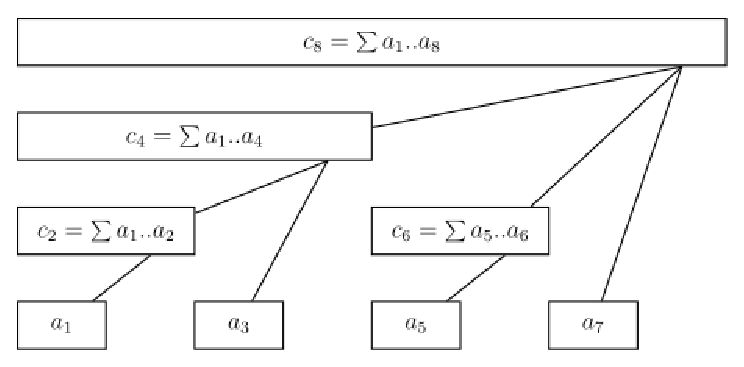
\includegraphics[width=\linewidth]{images/fenwick.eps}
  \caption{树状数组的示意图}
\end{figure}
\subsubsection{复杂度分析}
\paragraph{时间复杂度} 单点修改与区间查询的复杂度,由于二进制的性质,均为$O(log\,n)$,且由于位运算的使用,这个数据结构的常数较小。预处理相当于对每个元素进行一次更新,故为为$O(n\,log\,n)$
\paragraph{空间复杂度} 虽然该数据结构引入了额外的存储空间,但由于$c[n]$与$s[n]$大小同阶,故占用内存仍然为$O(n)$,只是常数略大。
\subsubsection{适用范围与局限性}
考虑m个请求,则处理所有这m个请求所需的时间复杂度为$O(m\,log\,n)$,当$n$,$m$在同一个数量级时,其时间复杂度可视为$O(n\,log\,n)$,远优于朴素的$O(n^2)$的数据结构。

但是对于区间修改的操作,树状数组的复杂度仍然不够理想。我们想要更进一步,实现对区间修改更加友好的数据结构。

\subsection{块状数组}
\subsubsection{实现方式}
对于区间操作一种很直接的想法就是,把整体划分为若干个小块,对整块整体处理,零散块单独处理。块状数组就是利用分块思想处理区间操作的一种数据结构。这里我们考虑区间修改操作和区间求和操作。

块状数组把一个长度为$n$的数组划分为$a$块,每块长度为$\frac{n}{a}$。对于一次区间操作,对区间內部的整块进行整体的操作,对区间边缘的零散块单独暴力处理。这里,块数既不能太少也不能太多。如果太少,区间中整块的数量会很少,我们要花费大量时间处理零散块;如果太多,又会让块的长度太短,失去整体处理的意义。

一般来说,我们取块数为$\sqrt{n}$,这在复杂度分析部分将进行详细的说明。

初始化块状数组时,要先划定出每个块所占据的范围:
\begin{lstlisting}
int sq = sqrt(n);
for (int i = 1; i <= sq; ++i)
{
    st[i] = n / sq * (i - 1) + 1;
     // st[i]表示i号块的第一个元素的下标
    ed[i] = n / sq * i;
     // ed[i]表示i号块的最后一个元素的下标
};
ed[sq] = n;
 //剩余的元素纳入最后一块中
for (int i = 1; i <= sq; ++i)
    size[i] = ed[i] - st[i] + 1;
 // 预处理每个块的大小
\end{lstlisting}
之后,对每个元素确定其所属的分块:
\begin{lstlisting}
for (int i = 1; i <= sq; ++i)
    for (int j = st[i]; j <= ed[i]; ++j)
        bel[j] = i; // 表示j号元素归属于i块
\end{lstlisting}
然后就可以读入数据,并对数据进行预处理:
\begin{lstlisting}
for (int i = 1; i <= n; ++i)
    A[i] = read(); // A[i]为原始数据
for (int i = 1; i <= sq; ++i)
    for (int j = st[i]; j <= ed[i]; ++j)
        sum[i] += A[j];
        // sum[i]保存第i个块的和
\end{lstlisting}
 
\paragraph{进行区间修改时} 当$x$与$y$在同一块内时,直接暴力修改原数组和\lstinline{sum}数组:
\begin{lstlisting}
if (bel[x] == bel[y])
    for (int i = x; i <= y; ++i)
    {
        A[i] += k;
        sum[bel[i]] += k;
    };
\end{lstlisting}
否则,先暴力修改左右两边的零散区间,然后对中间的整块打上标记:
\begin{lstlisting}
for (int i = x; i <= ed[bel[x]]; ++i)
{
    A[i] += k;
    sum[bel[i]] += k;
};
for (int i = st[bel[y]]; i <= y; ++i)
{
    A[i] += k;
    sum[bel[i]] += k;
};
for (int i = bel[x] + 1; i < bel[y]; ++i)
    mark[i] += k;
\end{lstlisting}

\paragraph{进行区间查询时} 如果左右两边在同一块,直接暴力计算区间和:
\begin{lstlisting}
if (bel[x] == bel[y])
    for (int i = x; i <= y; ++i)
        s += A[i] + mark[bel[i]]; 
        // 注意要加上标记
\end{lstlisting}
否则,暴力计算零碎块,再处理整块:
\begin{lstlisting}
for (int i = x; i <= ed[bel[x]]; ++i)
    s += A[i] + mark[bel[i]];
for (int i = st[bel[y]]; i <= y; ++i)
    s += A[i] + mark[bel[i]];
for (int i = bel[x] + 1; i < bel[y]; ++i)
    s += sum[i] + mark[i] * size[i]; 
    // 注意标记要乘上块的长度
\end{lstlisting}

\subsubsection{复杂度分析}
\paragraph{时间复杂度} 在最坏情况下,我们要处理接近个$\sqrt{n}$整块,还要对长度为$\frac{2n}{\sqrt{n}}$的零散块单独处理,故时间复杂度为$O(\sqrt{n})$。
\paragraph{空间复杂度} 虽然该数据结构引入了额外的存储空间,但由于$sum$等数组比$A$小($O(\sqrt{n})$),故占用内存仍然为$O(n)$,只是常数略大。
\subsubsection{适用范围与局限性}
分块的时间复杂度比不上树状数组这些对数级算法,但其可以支持的操作无需满足一些特殊的性质(比如结合律等),因而对于某些树状数组和后面的各种算法都无法支持的特殊的区间操作,使用块状数组是性能较好的选择。

\subsection{线段树}

\subsection{Chtholly树}

\section{总结}



\section{一级标题}

对投稿的基本要求:

(1)研究性论文主体应包括引言(重点论述研究的科学问题、意义、解决思路、价值、
贡献等)、相关工作(为与引言部分独立的一个章节)、主要成果论述、关键实现技术、
验证(对比实验或理论证明)、结论(结束语)等内容;系统实现或实验应有关键点的详细论述,以便读者能够重复实现论文所述成果。实验应有具体的实验环境设置、全面细致的数据对比分析。

(2)综述应包括引言、问题与挑战、研究现状分析、未来研究方向、结论等内容。以分析、对比为主,避免堆砌文献或一般性介绍、叙述。

(3)定理证明、公式推导、大篇幅的数学论述、原始数据,放到论文最后的附录中。

稿件提交时的基本要求:

(1)本模板中要求的各项内容正确齐全,无遗漏;

(2)语句通顺,无中文、英文语法错误,易于阅读理解,符号使用正确,图、表清晰无误;

(3)在学术、技术上,论文内容正确无误,各项内容确定。

\subsection{二级标题}

\subsubsection{三级标题}

正文部分, 字体为5号宋体。

文件排版采用 TeX Live。

正文文字要求语句通顺,无语法错误,结构合理,条理清楚,不影响审稿人、读者阅读理解全文内容。以下几类问题请作者们特别注意:

1)文章题目应明确反映文章的思想和方法;文字流畅,表述清楚;

2)中文文字、英文表达无语法错误;

3)公式中无符号、表达式的疏漏,没有同一个符号表示两种意思的情况;

4)数学中使用的符号、函数名用斜体;

5)使用的量符合法定计量单位标准;

6)矢量为黑体,标量为白体;

7)变量或表示变化的量用斜体;

8)图表规范,量、线、序无误,位置正确(图表必须在正文中有所表述后出现,即…如图1所示)(注意纵、横坐标应有坐标名称和刻度值)。

9)列出的参考文献必须在文中按顺序引用,即参考文献顺序与引用顺序一致,各项信息齐全(格式见参考文献部分);

10)首次出现的缩写需写明全称,首次出现的符号需作出解释。

11)图的图例说明、坐标说明全部用中文或量符号。

12)图应为矢量图。

13)表中表头文字采用中文。

14)公式尺寸:

标准:10.5磅

下标/上标:5.8磅

次下标/上标:4.5磅

符号:16磅

次符号:10.5磅

15)组合单位采用标准格式,如:“pJ/bit/m4”应为“\si{pJ/(bit.m^4)}”


\begin{theorem}
  定理内容。
  “定义”、“假设”、“公理”、“引理”等的排版格式与此相同,详细定理证明、公式可放在附录中。
\end{theorem}

\begin{proof}
  证明过程.
\end{proof}

\begin{figure}[htb]
  \centering
  \includegraphics[width=\linewidth]{example-fig.pdf}
  \caption{图片说明 *字体为小 5 号,图片应为黑白图,图中的子图要有子图说明*}
\end{figure}

\begin{table}[htb]
  \centering
  \caption{表说明}
  \small
  \begin{tabular}{cc}
    \toprule
    示例表格 & 第一行为表头,表头要有内容 \\
    \midrule
             &                            \\
    \midrule
             &                            \\
    \bottomrule
  \end{tabular}
\end{table}

\begin{procedure}
  \caption{过程名称}
  \small
  \begin{algorithmic}
    \REQUIRE
    \ENSURE
    \STATE \COMMENT{《计算机学报》的方法过程描述字体为小5号宋体,IF 、THEN等伪代码关键词全部用大写字母,变量和函数名称用斜体}
  \end{algorithmic}
\end{procedure}

\begin{algorithm}
  \caption{算法名称}
  \small
  \begin{algorithmic}
    \REQUIRE $n \geq 0 \vee x \neq 0$
    \ENSURE $y = x^n$
    \STATE $y \leftarrow 1$
    \IF{$n < 0$}
    \STATE $X \leftarrow 1 / x$
    \STATE $N \leftarrow -n$
    \ELSE
    \STATE $X \leftarrow x$
    \STATE $N \leftarrow n$
    \ENDIF
    \WHILE{$N \neq 0$}
    \IF{$N$ is even}
    \STATE $X \leftarrow X \times X$
    \STATE $N \leftarrow N / 2$
    \ELSE[$N$ is odd]
    \STATE $y \leftarrow y \times X$
    \STATE $N \leftarrow N - 1$
    \ENDIF
    \ENDWHILE
  \end{algorithmic}
\end{algorithm}



\begin{acknowledgments}
  致谢内容。
\end{acknowledgments}


\nocite{*}

\bibliographystyle{cjc}
\bibliography{example}


\newpage

\appendix

\section{}

附录内容置于此处,字体为小5号宋体。附录内容包括:详细的定理证明、公式推导、原始数据等


\makebiographies


\begin{background}
  *论文背景介绍为英文,字体为小5号Times New Roman体*

  论文后面为400单词左右的英文背景介绍。介绍的内容包括:

  本文研究的问题属于哪一个领域的什么问题。该类问题目前国际上解决到什么程度。

  本文将问题解决到什么程度。

  课题所属的项目。

  项目的意义。

  本研究群体以往在这个方向上的研究成果。

  本文的成果是解决大课题中的哪一部分,如果涉及863/973以及其项目、基金、研究计划,注意这些项目的英文名称应书写正确。
\end{background}

\end{document}
